\chapter{Design}
\label{ch:design}
In this chapter we will design the data structure of our test data,
as well as the workloads to simulate a typical industrial use of our examined databases.

After that we will plan our extension for YCSB in section~\ref{ch:design:se:extensionOfTheBenchmark},
both for the internals of the benchmark and the bindings to connect the databases.

In the end in section~\ref{ch:design:se:executionTool} and~\ref{ch:design:se:evaluationTool} we will outline tools to support execution of the benchmark and evaluation of the results.

\section{Data Structure}
\label{ch:design:se:dataStructure}
To create a schema for our data structure we had a meeting with other researchers at our institute.
The result of out session can be seen in figure~\ref{fig:firstDesignOfSchema}.
In the centre left we see "Features of Interest" which could be mapped to the "testFeature" edge in the industrial example of figure~\ref{fig:exampleData} as it depicts an observation of some product.
At the bottom we see a "M" which stands for "Machine",
its connection to "P. Schritte"\footnote{german for production steps} shows that this machine does one to n production steps.
Every production step is associated with a component which consists of a PCB\footnote{short for printed circuit board} what has different parts,
a version and a file after which it was created.

As the model shows too much detail in some areas without giving a good overview of an industrial data schema,
we had to reiterate over it and get rid of some complexity where we don't need it for our purposes.

\begin{figure}
  \centering
  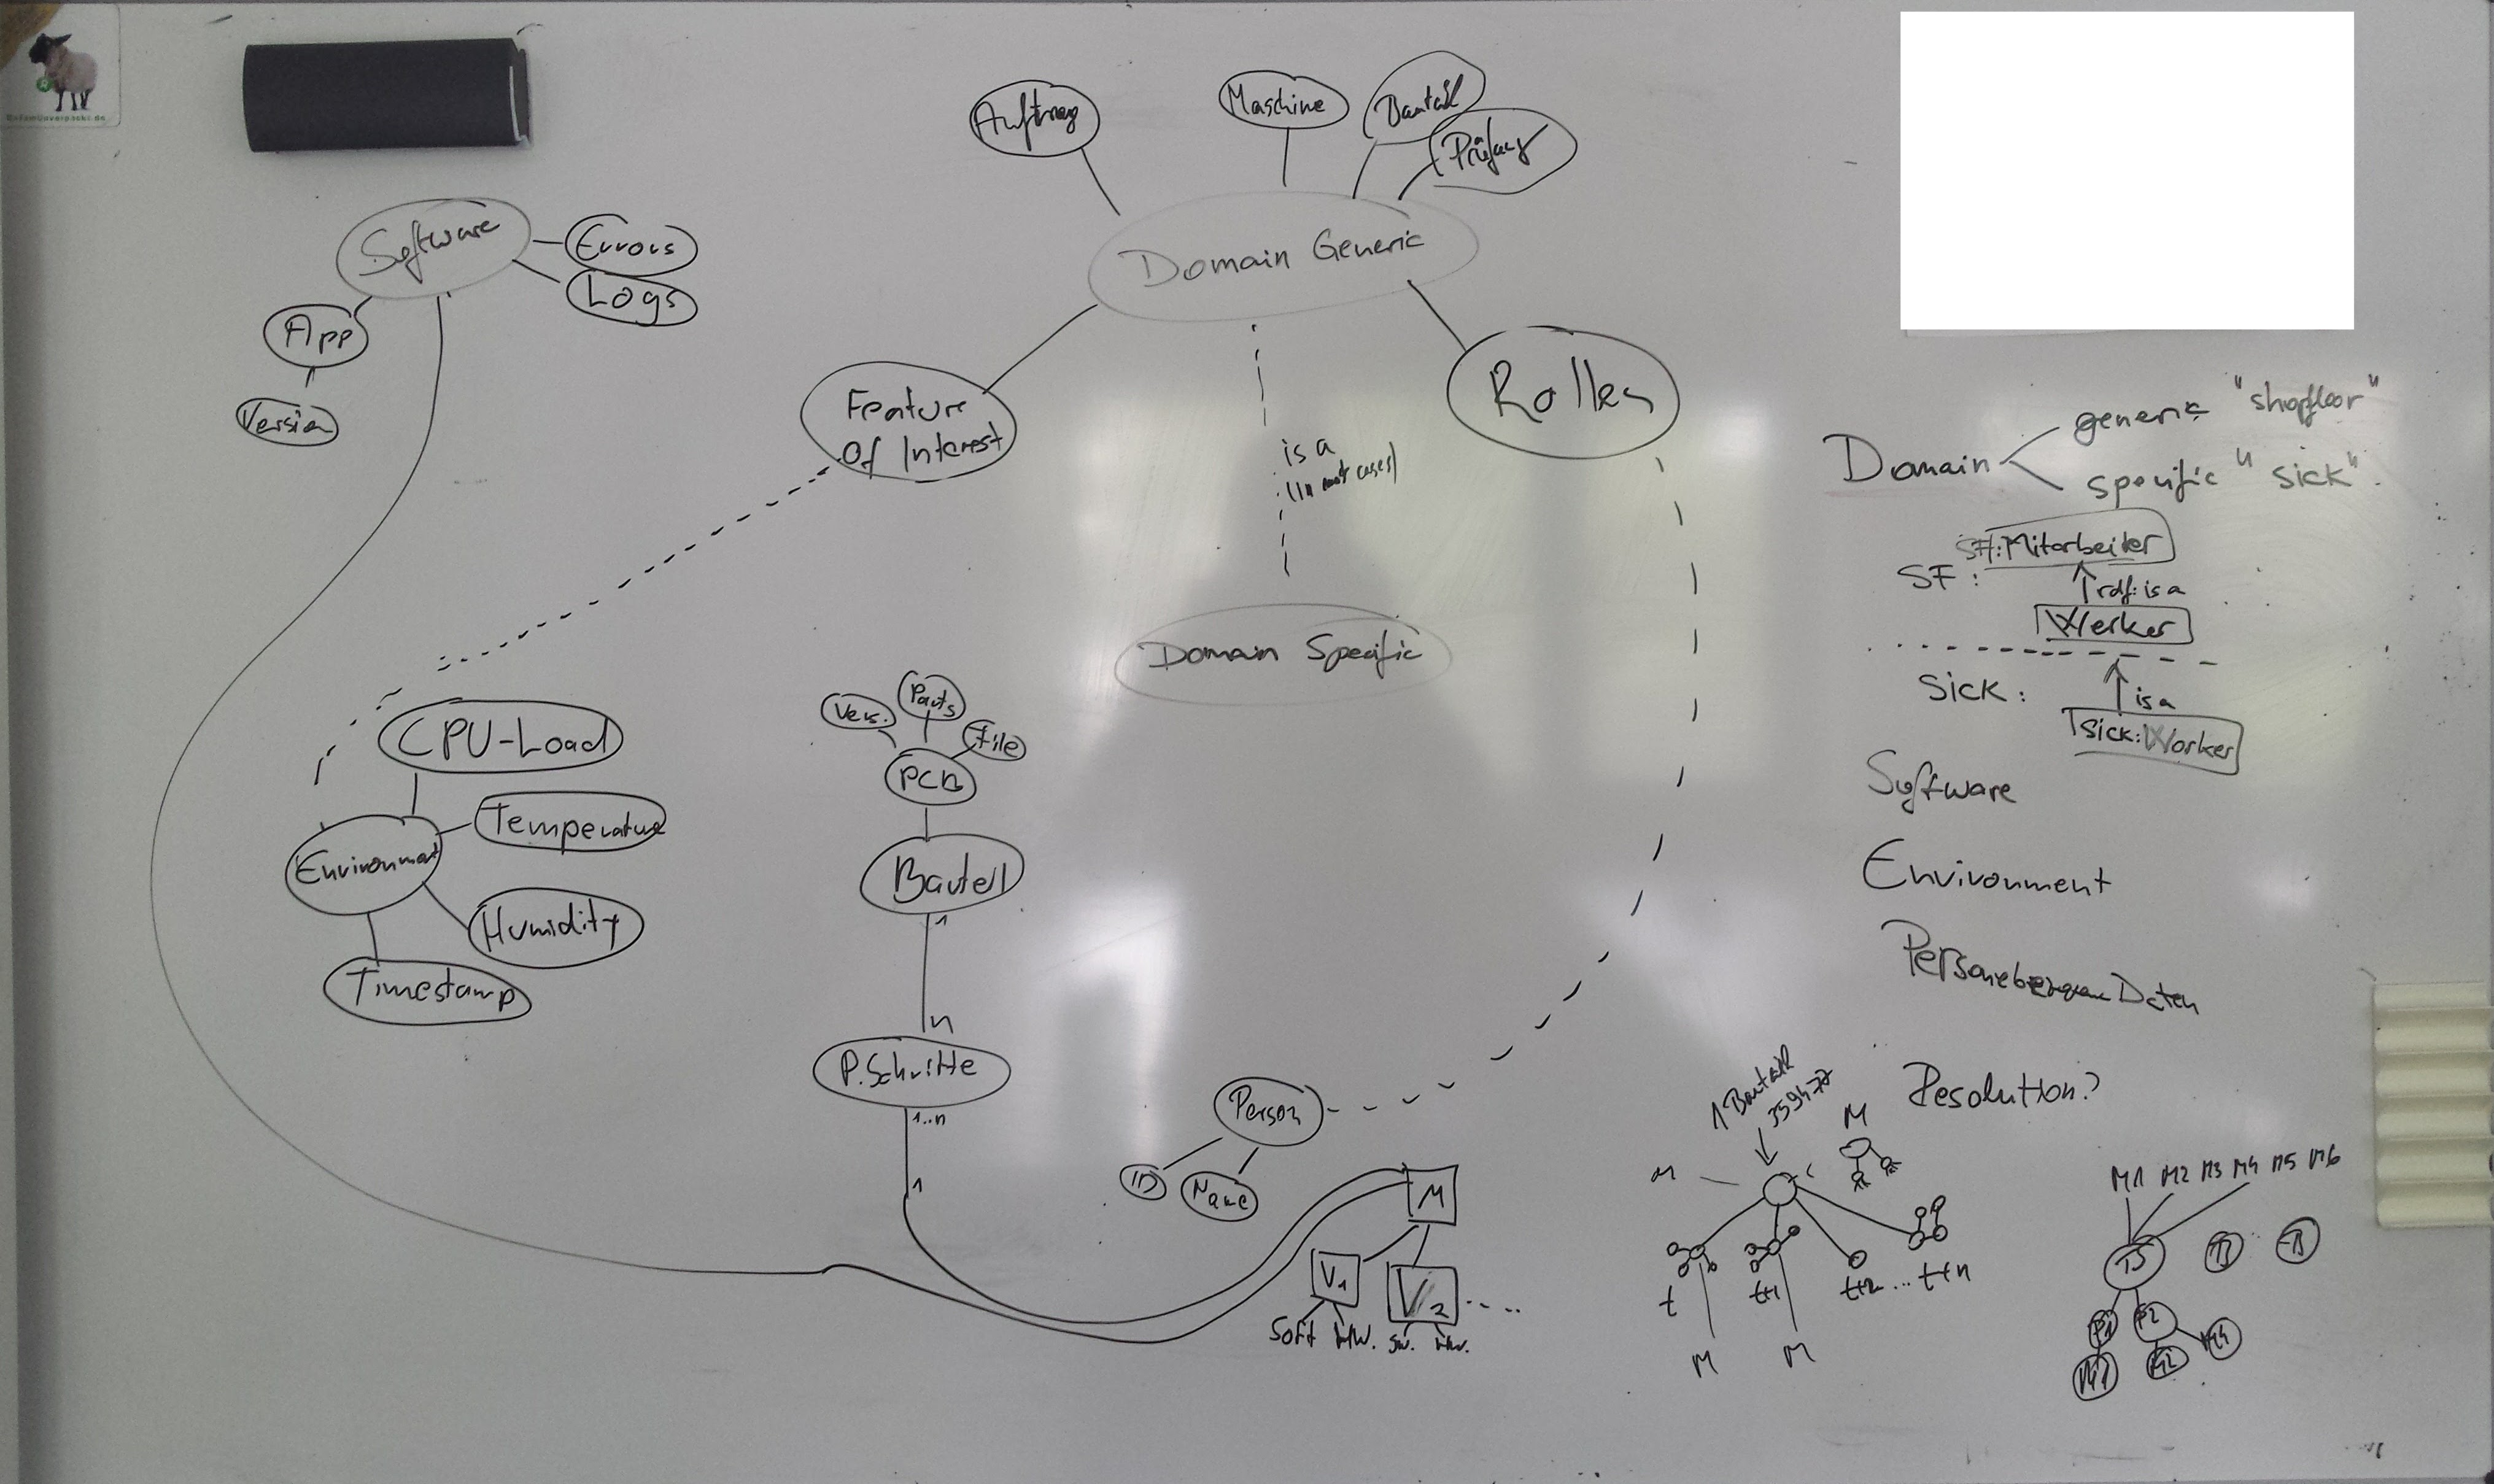
\includegraphics[width=\textwidth]{images/firstDesignOfSchema}
  \caption{The first design of a data schema for industrial data. Created by researchers at our institute.}
  \label{fig:firstDesignOfSchema}
\end{figure}

The meeting gave us a better understanding of how a production facility could handle its data and with that in mind and the objective to design a simpler schema that includes to most necessary parts of production the model shown in figure~\ref{fig:finalDesignOfSchema} was created.

\begin{figure}
  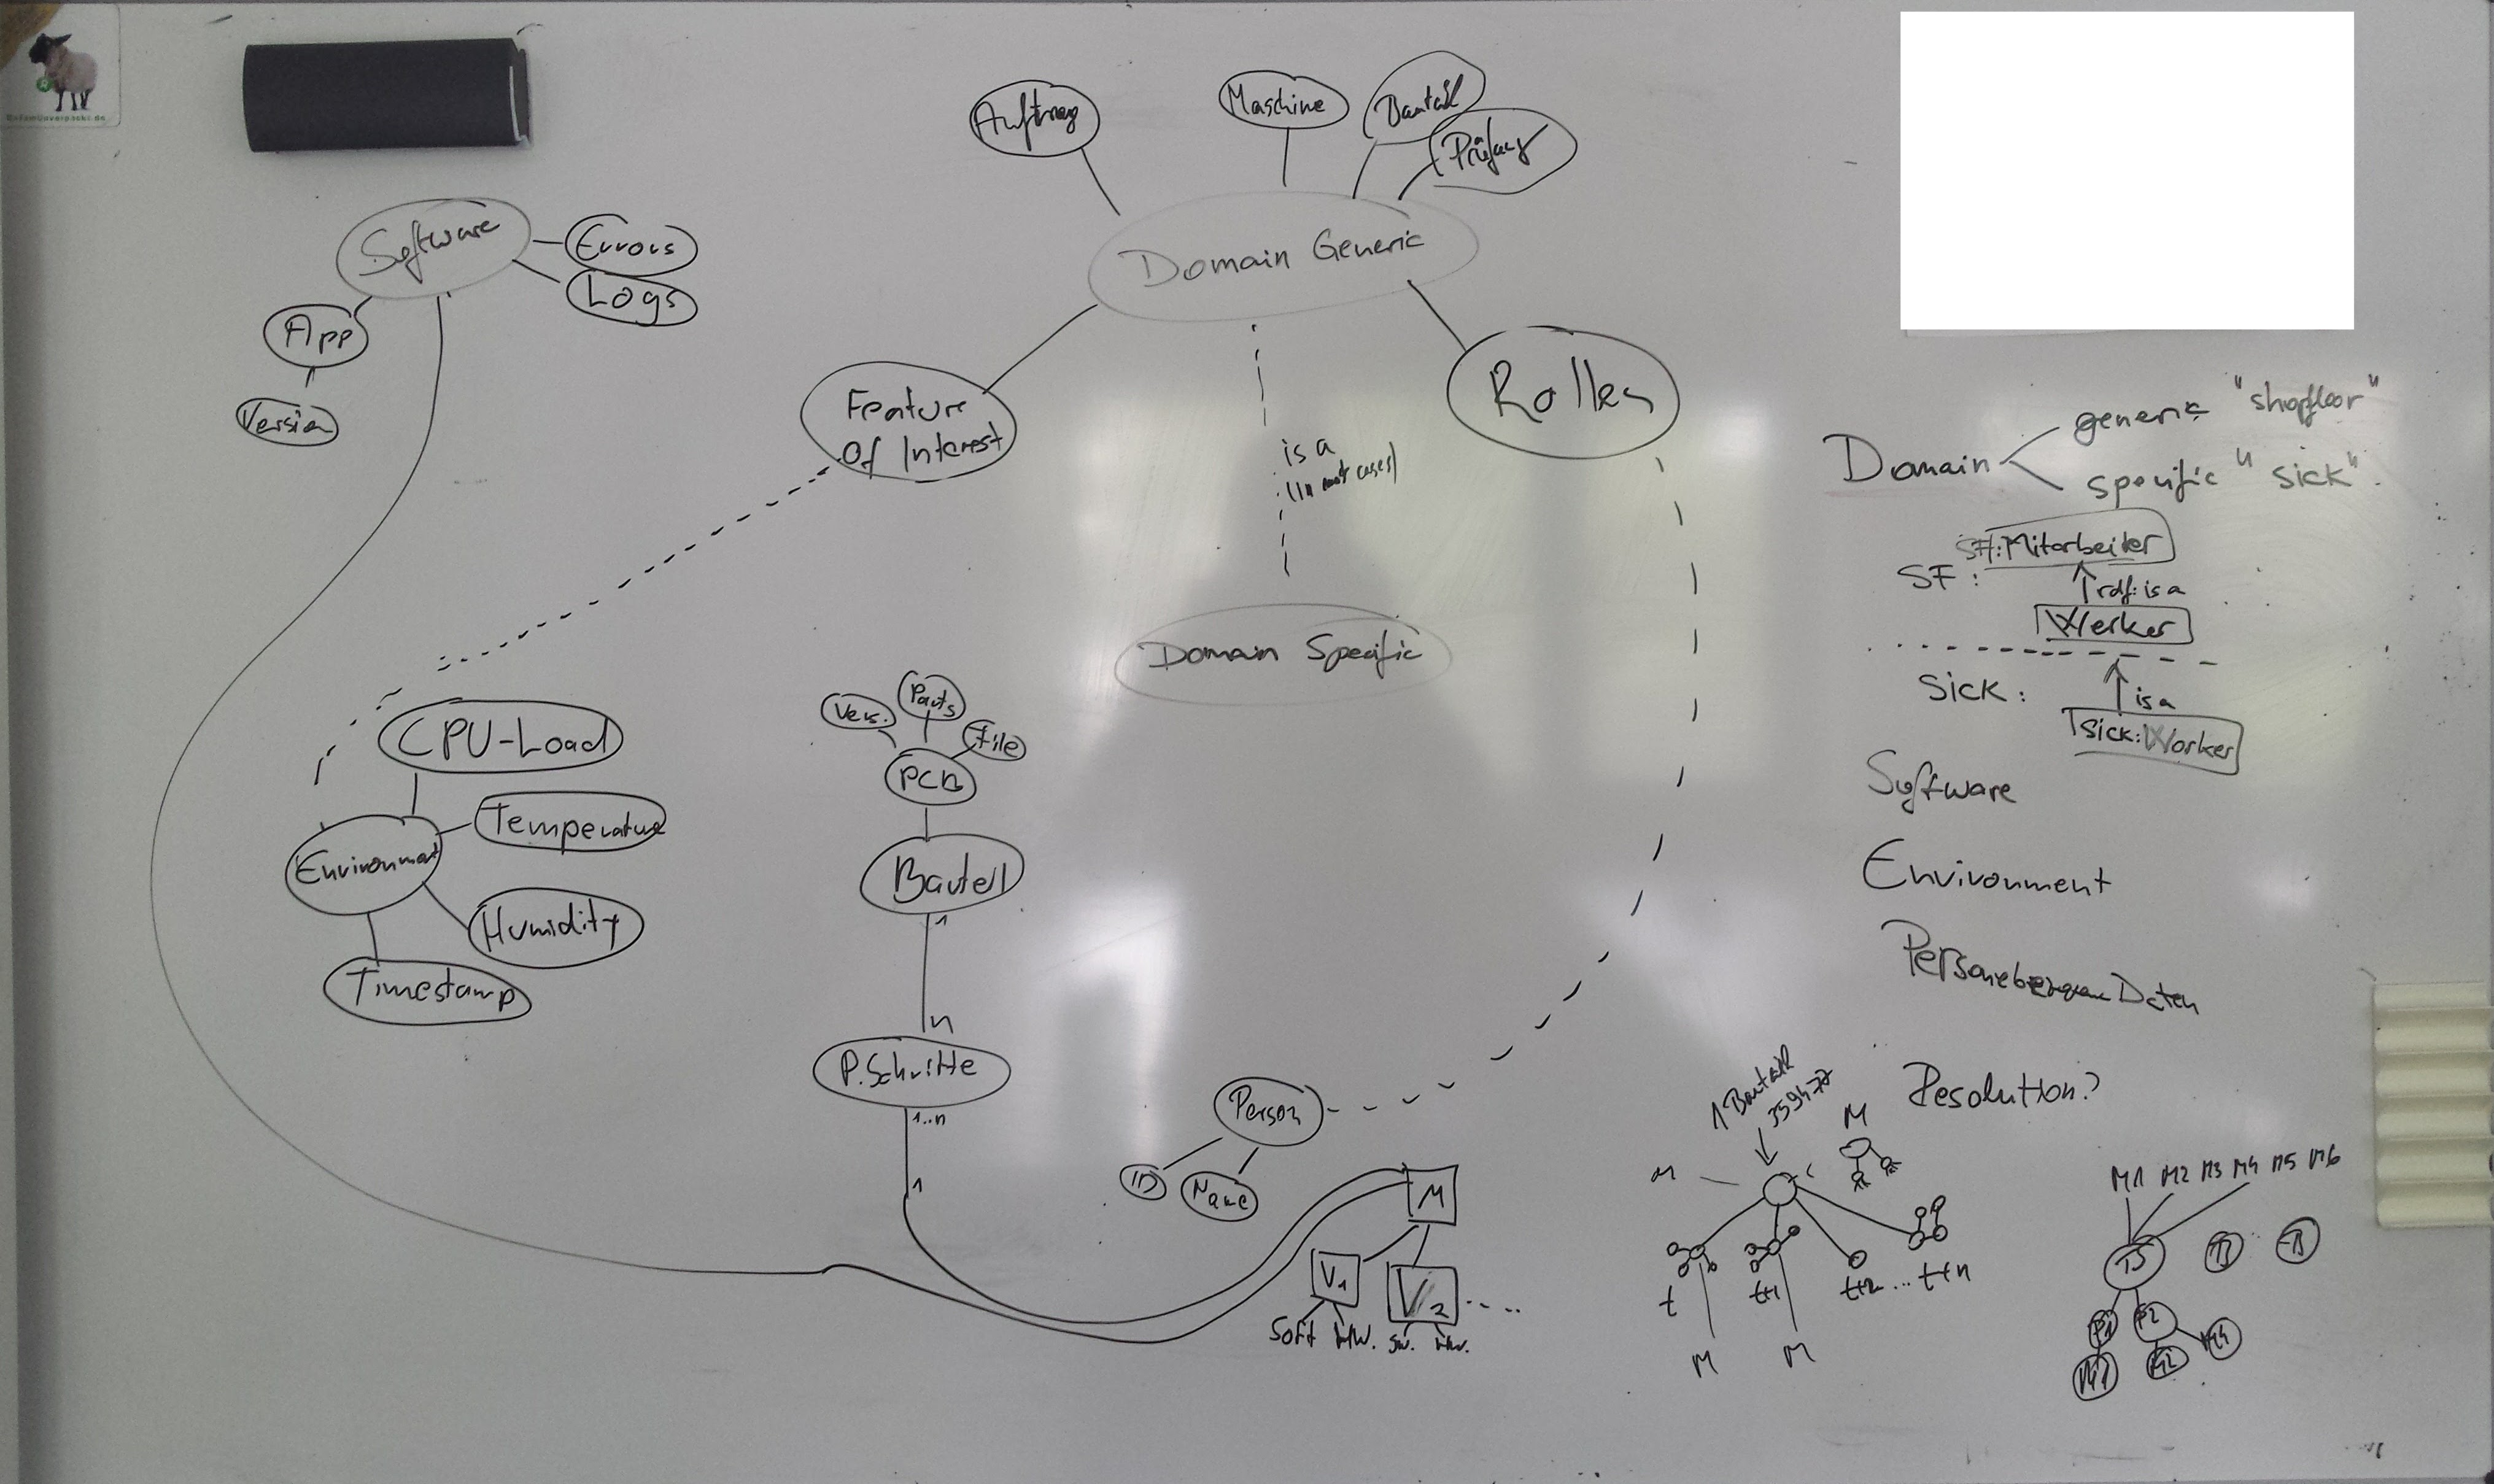
\includegraphics[width=\textwidth]{images/firstDesignOfSchema}
  \caption{The final design of the data schema.\todo{figure with final data structure as implemented}}
  \label{fig:finalDesignOfSchema}
\end{figure}

\todo{create graphic and describe its content. Graphic should have numbers on its edges, maybe use puml. Naming of parameters}

\section{Workloads}
\label{ch:design:se:workloads}
Our workload design will be separated into three part.
In subsection~\ref{ch:design:se:throughput} we discuss the design of workloads aimed to uncover the ability to store large amounts of data.
Subsection~\ref{ch:design:se:productionSimulation} will directly investigate the suitability of a database to be used in an industrial use case for storing data.
We will design workloads to examine the other industrial use case of retrieving data under load in subsection~\ref{ch:design:se:retrievingUnderLoad}.
Finally we will give a summary over all workloads we are going to run on the databases in subsection~\ref{ch:design:se:summary}

\subsection{Throughput}
\label{ch:design:se:throughput}
To explore the throughput of the databases we will have some variables we will change over the course of the different workloads.
These variables are

\begin{itemize}
  \item using an index on the key
  \item the size of a single property of the node
  \item using no edges with an index.
\end{itemize}

The last variable sound counter intuitive,
since edges add meaning to the data,
but by eliminating them we want so see if edges could be a cause of delay,
because to add an edge the start and end node need to be known and therefore be retrieved at first.

We will go over the different variables in the following subsections and motivate their purpose.

\subsubsection{Index}
\label{ch:design:se:index}
For this category we will use different data set sizes in terms of their number of nodes.
We will use steps of multiplication by 10 from 1.000 nodes to 10.000.000 nodes,
to examine if there is a linear correlation between the number of nodes and the time needed to store them.

Switching from indexed to not indexed we want to inspect how write speed or operations per second are effected.
Indexing is important to retrieve data more quickly for the cost of write speed,
with this workload we will see if the sacrifice in write speed is reasonable.
We will only use an index on the node and edge key,
which will be used to search that graph component\footnote{a node or an edge of the graph} in the database.
Indexing the other properties would have no benefit in our example. \note{would have, e.g. temperature of component. Results could be mapped to those.}

For this workload we will use a node property size of 10B,
that is small enough to not have an impact on performance but large enough to represent most of the data stored in the properties of our example.

\subsubsection{Node Property Size}
\label{ch:design:se:nodePropertySize}
After retrieving a number of nodes that represents a acceptable execution time we will vary the next variable which is the property size.
We will go from 10B used in the index benchmarks to up to 1MB,
again in steps of multiplying by 10 (10B, 100B, 1KB, ..., 1MB).

The typical property size is between 1B (1 character) and roughly 75B (75 characters) according to our example in listing~\ref{lst:exampleData}.

The use of properties is not limited to short strings,
that is why we will investigate if larger amounts of data influence the throughput more than linearly.

We will use an index on the keys,
because using an index would represent the use in the industry and since we are not indexing the growing values there will be no impact from using it.

\subsubsection{No Edges}
\label{ch:design:se:noEdges}
\note{maybe remove index, as it has no real purpose. Underline importance of investigating the speed difference without edges. Maybe indexing helps, make sure to compare both with the workloads with edges to see if index helps with edges.}
In subsection~\ref{ch:design:se:throughput} we already justified why we will investigate the throughput with an exclusive use of nodes in the data set.

As this workload does not allow for much variation besides using an index or not,
it will only include these two workloads.

As in subsection~\ref{ch:design:se:nodePropertySize} we will use a suitable large data set in terms of node count resulting from the first workloads.
We will use the same node size as in~\ref{ch:design:se:index} to be able to compare the results directly to the corresponding ones from that workload.

\subsection{Production Simulation}
\label{ch:design:se:productionSimulation}
Related to production we will investigate the impact of the structure and the general suitability for an industrial use.
The next two subsection will cover those aspects in more detail.

The property size will be set to 50B,
which should be enough to cover on average most values stored in the database.

\subsubsection{Structure}
For production we have some variables to investigate which mainly effect the structure of our data.
We have three layers which we can blow up horizontally by increasing the corresponding parameters,
which are

\begin{itemize}
  \item \note{maybe link to figure if suitable}
  \item productsperorder, this spreads the data graph apart at a level closer to the root
  \item componentsperproduct, this changed the width in the middle of the graph
  \item testparametercount, which widens the graph at the lowest level.
\end{itemize}

For production simulation we will first examine if the data structure impacts performance of the databases.
To investigate this aspect we will change the width of the graph with the variables mentioned above.
We will use the numbers from section~\ref{ch:analysis:se:data} as the maximum width,
which would be $ productsperorder = 64 $, \linebreak
$ componentsperproduct = 128 $ and $ testparametercount = 128 $.
In the first workload we will set all variables to one,
the next one will use $ productsperorder = 16 $, $ componentsperproduct = 32 $ and $ testparametercount = 32 $.
The third and last one will use the maximum width mentioned above.
By this variation we will cover the minimum and maximum with an additional result in the middle to see if there are any changes in performance.

The keys of the graph components will be indexed,
because indexing these values should be done to later work on that data more efficiently,
which is necessary for the industry.

\subsubsection{Suitability}
To examine if a database is suitable for the industry it should be able to store the data faster then it is coming from the machines.
In section~\ref{ch:analysis:se:dataAmount} we calculated that 1.056.833 nodes would be written to the database every three minutes.
First we will set up a data set with that amount of nodes and insert it into the database,
that will allow us to compare the time needed to store all data with our three minute limit.
If the database should take more than three minutes it would not be suitable,
since data is produced faster than it can be stored.

The next steps would be to repeat that procedure with a node amount that represents a whole hour, day, week, month and year,
iff the databases are storing the data fast enough to not take up an unreasonable amounts of time in running the benchmark.

We will use the structure with the maximum width,
because it represents the industrial use case best regarding the information given by our partners at SICK AG~\cite{SICK}.

\subsection{Retrieving under load}
\label{ch:design:se:retrievingUnderLoad}
\todo{mention potential to compare to other studies.}
There would be no point in storing data if it is not retrieved at some point.
To investigate on the performance of reading and scanning (more on that in subsection~\ref{ch:design:se:scanning}) data from the database the following workloads are designed.

As mentioned in section~\ref{ch:design:se:index} indexing is important for retrieving data,
therefore we will us it as a variable for this workload category.
By doing so we want to examine if the price we pay while writing is justified by the performance gain in retrieving data.

The node amount will be determined by the first workload investigating the throughput,
to not take up too much time testing these features.

We want to retrieve both nodes and edges,
because either could be useful,
since the edges can also store properties in them.

\subsubsection{Reading}
\label{ch:design:se:reading}
Reading single values is the basic operation when it comes to retrieving data from a database.
Since the database will be under constant load,
because of production delivering data all the time,
we will use $ 5\% $ of the total operations executed in this workload for read operations,
the rest will be inserting data.

\subsubsection{Scanning}
\label{ch:design:se:scanning}
Scanning a graph can be done in multiple ways,
the simplest being depth first search~\cite{Tarjan1972},
to retrieve values associated with connected nodes.
For example you could scan from a machine to get the test features of their produced products.

As in subsection~\ref{ch:design:se:reading} we will use a mix of $ 5\% $ scan operations with $ 95\% $ insert operations,
to simulate the constant load present in an industrial environment.

The number of steps to do during scanning will be $ 1000 $ as that was the default value set in YCSB and it should also represent a good amount of data to read.

\subsection{Summary}
\label{ch:design:se:summary}
In this subsection we will give an overview over all workloads and their variables.

For the workloads measuring the throughput "Products per Order",
"Components per Product" and "Test Parameter Count" will all be set to $ 1 $.
Their overview is shown in table~\ref{tab:throughput}

\begin{table}[!h]
  \begin{minipage}{\textwidth}
    \begin{tabularx}{\textwidth}{ | X | X | X | X | X | }
      \hline
      Aspect & Node Count & Node Size & Index & Only Nodes \\ \hline
      1. With Index & 1.000 & 10B & True & False \\ \hline
      2. With Index & 10.000 & 10B & True & False \\ \hline
      3. With Index & 100.000 & 10B & True & False \\ \hline
      4. With Index & 1.000.000 & 10B & True & False \\ \hline
      5. With Index & 10.000.000 & 10B & True & False \\ \hline
      1. Without Index & 1.000 & 10B & False & False \\ \hline
      2. Without Index & 10.000 & 10B & False & False \\ \hline
      3. Without Index & 100.000 & 10B & False & False \\ \hline
      4. Without Index & 1.000.000 & 10B & False & False \\ \hline
      5. Without Index & 10.000.000 & 10B & False & False \\ \hline
      1. Node Size & x & 100B & True & False \\ \hline
      2. Node Size & x & 1KB & True & False \\ \hline
      3. Node Size & x & 10KB & True & False \\ \hline
      4. Node Size & x & 100KB & True & False \\ \hline
      5. Node Size & x & 1MB & True & False \\ \hline
      1. No Edges & x & 10B & True & True \\ \hline
      2. No Edges & x & 10B & False & True \\ \hline
    \end{tabularx}
  \end{minipage}
  \caption{Workloads to investigate the throughput. x is a placeholder for a suitable data set size in terms of execution time.}
  \label{tab:throughput}
\end{table}

The workloads to investigate the suitability for the industry are shown in table~\ref{tab:productionSimulation}.
For these workloads the property size is fixed to 50B and an index is used on all workloads.
Edges are also used in these workloads to reflect the use in the industry.

\begin{table}[!h]
  \begin{minipage}{\textwidth}
    \begin{tabularx}{\textwidth}{ | X | X | X | X | X | }
      \hline
      Aspect & Node Count & Products per Order & Components per Product & Test Parameter Count \\ \hline
      1. Structure & x & 1 & 1 & 1 \\ \hline
      2. Structure & x & 16 & 32 & 32 \\ \hline
      3. Structure & x & 64 & 128 & 128 \\ \hline
      1. Suitability (three minutes) & 1.056.833 & 64 & 128 & 128 \\ \hline
      2. Suitability (hour) & 21.136.660 & 64 & 128 & 128 \\ \hline
      3. Suitability (day) & 507.279.840 & 64 & 128 & 128 \\ \hline
      4. Suitability (week) & 3.550.958.880 & 64 & 128 & 128 \\ \hline
      5. Suitability (month) & 15.218.395.200 & 64 & 128 & 128 \\ \hline
      6. Suitability (year) & 185.157.141.600 & 64 & 128 & 128 \\ \hline
    \end{tabularx}
  \end{minipage}
  \caption{Workloads to simulate production. Again x represents a placeholder for a suitable data set size.}
  \label{tab:productionSimulation}
\end{table}

The remaining workloads to examine the ability to retrieve data are shown in table~\ref{tab:retrievingUnderLoad}.
These workloads will use a appropriate data set size regarding execution time and a property size as in the production simulation of 50B.
A simple structure is used to investigate the basic capabilities of data retrieval,
that means "Products per Order",
"Components per Product" and "Test Parameter Count" are set to $ 1 $.

\begin{table}[!h]
  \begin{minipage}{\textwidth}
    \begin{tabularx}{\textwidth}{ | X | X | X | X | X | }
      \hline
      Aspect & Index & Insert Proportion & Read Proportion & Scan Proportion \\ \hline
      1. Reading & True & 95\% & 5\% & 0\% \\ \hline
      2. Reading & False & 95\% & 5\% & 0\% \\ \hline
      1. Scanning & True & 95\% & 0\% & 5\% \\ \hline
      2. Scanning & False & 95\% & 0\% & 5\% \\ \hline
    \end{tabularx}
  \end{minipage}
  \caption{Workloads to investigate capability to retrieve data under load.}
  \label{tab:retrievingUnderLoad}
\end{table}

\section{Extension of the Benchmark}
\label{ch:design:se:extensionOfTheBenchmark}
To be able to execute the introduced workloads and use the data structure designed above,
we need to extend the YCSB benchmark.
For the benchmark to be able to execute our workloads the way we want them to be executed the following parts of the benchmark need to be extended

\begin{itemize}
  \item Generation of the dataset
  \item Generation of rondom graph components
  \item Generation of a operation order
  \item Workload to use the generated dataset
  \item Database bindings.
\end{itemize}

In the following subsections we will go in more detail over the different areas we are planing to modify.

\subsection{Graph Data Generator}
YCSB does not include a graph data generator,
therefore we need to create one that fulfils our needs.

The generator should create a data set with the structure mentioned in section~\ref{ch:design:se:dataStructure} and store the data for future reproduction when using the benchmark with the next database.

The two parts of the generator,
which are creating together with storing the data and recreating the data are designed in subsection~\ref{ch:design:se:storingTheDataset} and~\ref{ch:design:se:restoringTheDataset} respectively.

Generally to represent a graph in YCSB we need some classes to represent nodes, edges and the graph.
In section~\ref{ch:background:se:graphs} we mentioned that a graph is a tuple of a set of nodes and a set of edges.
That can be directly mapped to a class with two lists,
one for nodes and the other one for edges.
We want the nodes to have a key for identification,
a label to match it with an object that could exist in the real world and a value,
which will represent the data stored in the node,
the size of this value should be directly linked the the property size from~\ref{ch:design:se:nodePropertySize}.
An edge should also have a key for identification,
a label to add meaning to it and a start and an end node,
represented by their keys.

The generator of the dataset should decide if it should create a new one or recreate it by looking at the existing files.

\subsubsection{Storing the Dataset}
\label{ch:design:se:storingTheDataset}
\todo{Activity diagram of $ GraphDataRecorder::createGraph() $}
We want to control the size of the dataset with our variables mentioned in the workload section~\ref{ch:design:se:workloads} so this generator should create small subgraphs with only one node and its corresponding edges every time it is asked for a new value.
By storing the current state of the created graph in the generator class,
we can always determine the next subgraph to create.

The modify the structure of the graph with our three variables,
these need to be parsed in this class and used during subgraph creation.

An activity diagram is shown in figure~\ref{fig:dataCreation} to illustrate the creation process with usage of the parameters for tweaking the width of the graph.

\begin{figure}
  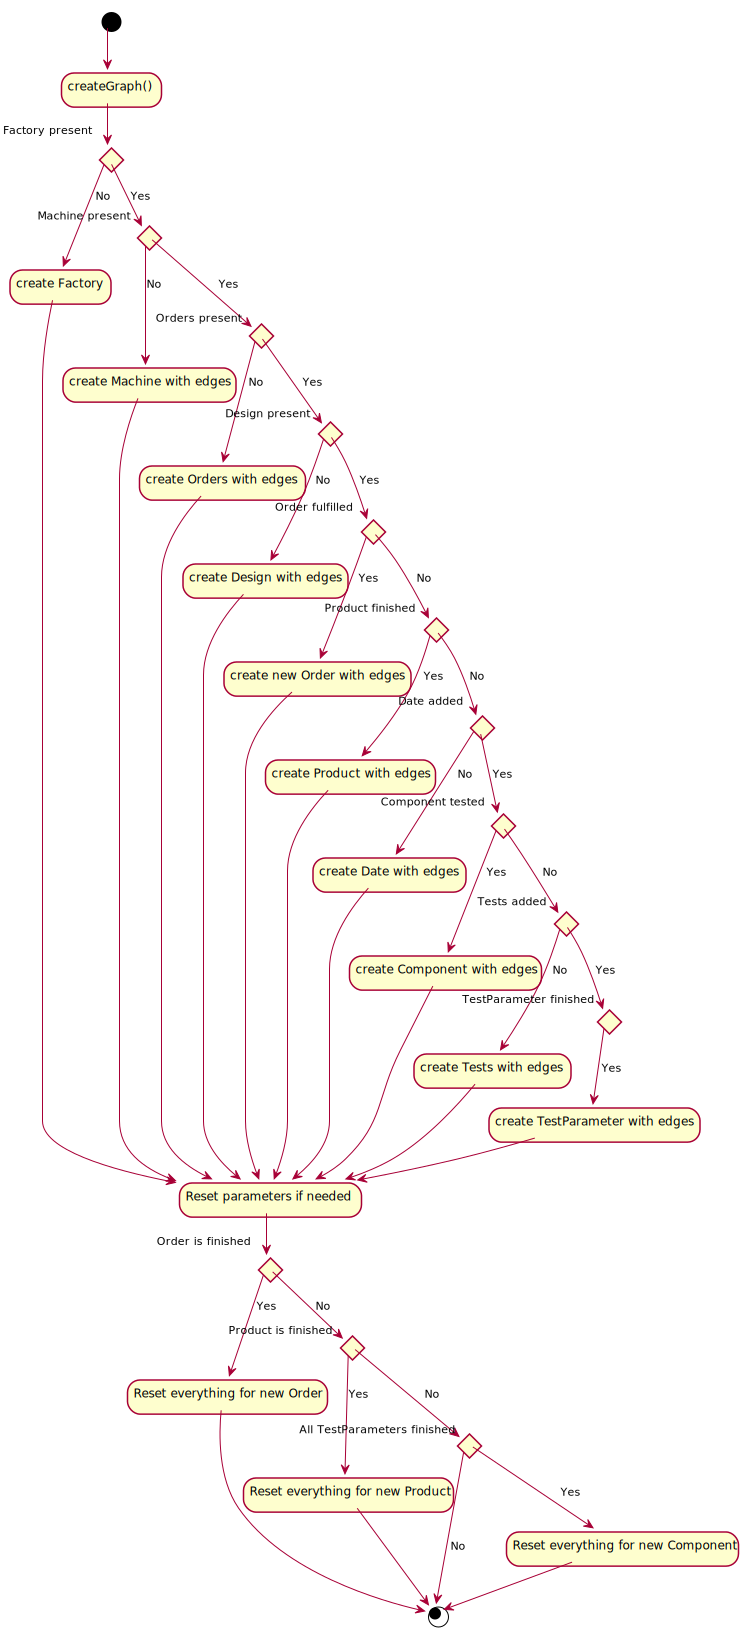
\includegraphics[width=\textwidth/2]{images/dataCreation}
  \caption{Activity diagram of the creation process for the dataset.\todo{create and describe}}
  \label{fig:dataCreation}
\end{figure}


To restore that data also one node at a time we will store each created subgraph in a file,
for that we will serialise the graph and deserialise it when we are restoring the data.

To disable edges for the workload from subsection~\ref{ch:design:se:noEdges} we can simply skip the step of creating and adding them to the graph.

\subsubsection{Restoring the Dataset}
\label{ch:design:se:restoringTheDataset}
The restoring of the data should be easily done by deserialising it from the created file during creation of the dataset.
Since the single subgraphs were stored in the file,
we can pass the to the workload just after deserialising them.

For larger datasets we should read the subgraphs from the file as needed and not at the beginning,
because that could fill up the RAM with the dataset and leave less memory for the database to work with.

\subsection{Random Graph Component Generator}
Reading and scanning operations require a point to start with in the data,
that's why we need the key of some component in the graph.
The kay can be randomly chosen,
but the node or edge associated with it has to be present in the database.
Therefore we need to somehow store the keys of the graph components we have already put into the database,
that could be done in the $ GraphDataGenerator $ created for subsection~\ref{ch:design:se:storingTheDataset},
because it anyway touches all created values.

Because we want to retrieve edges and nodes randomly we have to pick one of the two randomly every time a random component is required.
As in~\ref{ch:design:se:storingTheDataset} and its subsections,
every created value needs to be stored to be retrieved later on.
The data needed for this generator is not as complex as a graph and can therefore be stored directly in a file line by line for easy storing and restoring.
That also means,
that we can read the files at the beginning of the run so it is faster accessible during the benchmark without using to much memory.

For the workload which requires the absents of edges a method should be defined to return only a randomly chosen node.

Figure~\ref{fig:randomGraphComponentGenerator} shows an activity diagram of the generator.

\begin{figure}
  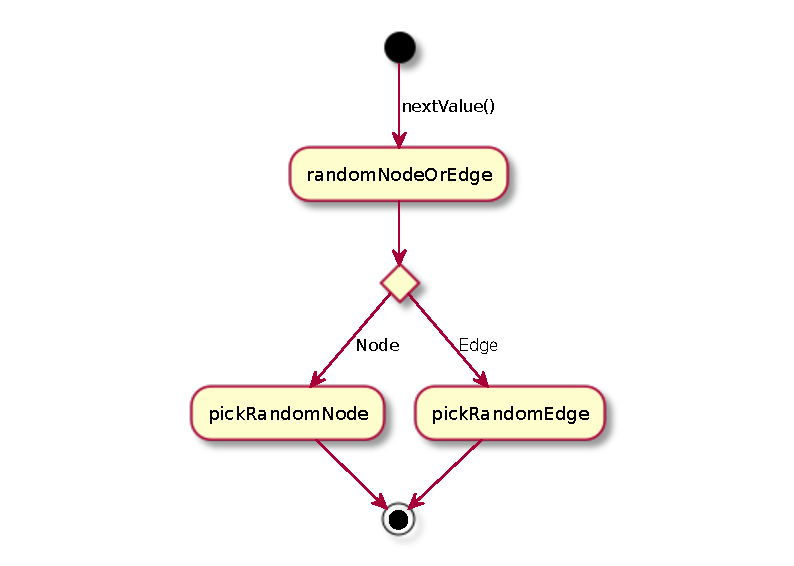
\includegraphics{images/randomGraphComponentGenerator}
  \caption{Activity diagram of the $ RandomGraphComponentGenerator $ showing the process of storing and restoring.\todo{}}
  \label{fig:randomGraphComponentGenerator}
\end{figure}

\subsection{Operation Order Generator}
\label{ch:design:se:operationOrderGenerator}
To fix the execution order of inserting and retrieving data to and from the graph,
we need to store the operations too.
That can be done by simply storing the name of each operation in a file as it appears and reading it from there when running the benchmark.

In YCSB there is already a $ DiscreteGenerator $\footnote{com.yahoo.ycsb.generator.DiscreteGenerator} which take a value and a weight and returns distributed according to the weights a value,
this can be used to get the operations to run on the database.

Figure~\ref{fig:operationOrderGenerator} visualises the procedure of storing the operation order.

\begin{figure}
  \includegraphics{images/operationOrderGenerator}
  \caption{Activity diagram of the operationOrderGenerator.\todo{}}
  \label{fig:operationOrderGenerator}
\end{figure}

\subsection{Graph Workload}
The $ GraphWorkload $s task is to coordinate the different generators and to execute the workload as specified.
To be able to store the generated dataset in a specific folder on the system the workload class should take a path to a folder and instrument the generators to store their data in that folder or recreate it from there respectively.

This class will be the interface between the client calling $ Workload::doInsert $ and $ Workload::doTransaction $ and the database.
The $ Workload::doInsert $ method will only insert a subgraph into the database,
to do so the workload class needs to get the subgraph from the GraphDataGenerator and redirect its value to the database.
For the $ Workload::doTransaction $ method the workload has to be able to call the available methods on a database which are

\begin{itemize}
  \item DB::insert(String table, String key, Map<String, ByteIterator> values)
  \item DB::read(String table, String key, Set<String> fields, Map<String, ByteIterator> result)
  \item DB::scan(String table, String key, int recordcount, Set<String> fields, Vector<HashMap<String, ByteIterator>{}> result)
  \item DB::update(String table, String key, Map<String, ByteIterator> values)
  \item DB::delete(String table, String key).
\end{itemize}

We will only use the first three for our workloads,
but the other ones should be implemented too,
to support future workloads.
To determine which operation should be executed the $ OperationOrderGenerator $ from subsection~\ref{ch:design:se:operationOrderGenerator} will be used.

In general we see,
that a $ table $ is given as an argument,
in a graph database we don't have tables as in relational databases,
so we can use it to distinguish between nodes and edges,
by simply passing the string "node" or "edge" to the database.
Next is a $ key $,
which we can use to pass the key identifier of the graph component to the database.
The $ values $ map will contain the values of the graph components to insert parsed into a map for compatibility and vice versa for the $ result $ map and vector.
Our data design does not focus to much on the individual properties the nodes and edges could have,
therefore we will simply read all $ fields $ of the graph component.

\textbf{DB::insert} \newline
As described above the $ DB::insert $ method will get a value from the \linebreak
$ GraphDataGenerator $ and insert it into the database.

\textbf{DB::read} \newline
The read operation will pick a random graph component with the \linebreak
$ RandomGraphComponentGenerator $ and use its kind (node or edge) as the $ table $ argument and the key identifier as the $ key $ argument.

\textbf{DB::scan} \newline
Scanning also requires a random component which will be chosen by the \linebreak
$ RandomGraphComponentGenerator $.
The mapping is also the same as with $ DB::read $ for the $ table $ and $ key $ arguments.
$ recordcount $ will be set to $ 1000 $ as that is the default value specified by the $ CoreWorkload $\footnote{com.yahoo.ycsb.workloads.CoreWorkload} and that value represents a good amount for scanning.

\textbf{DB::update} \newline
For this operation we need a randomly picked graph component from the \linebreak
$ RandomGraphComponentGenerator $ to get a valid key identifier.
Only the property value should be changed during update,
not the identifier nor the label,
that means that only nodes will be changes,
as edges have no property value assigned to them.

\textbf{DB::delete} \newline
This takes a random graph component via the $ RandomGraphComponentGenerator $ and calls the $ delete $ method of the database.

To avoid calling these methods with edges when the workload specifies to not use them,
a parameter which can be set should determine if a random graph component or a random node should be picked by the $ RandomGraphComponentGenerator $.

Since the client only calls $ Workload::doTransaction $ to execute one of the various database operations the $ OperationOrderGenerator $ should be called to generate the next operation.

\subsection{Bindings}
\label{ch:design:se:bindings}
To ensure compatibility with other workloads present in YCSB we will extend the $ DB $ class and implement the methods used for other databases.
Because graph databases are slightly different we will explain how each database will map the arguments of the $ DB $ methods to their own API in the following subsections.

The basic functions we need from our database are

\begin{enumerate}
  \item creating a node
  \item creating an edge
  \item adding properties to a node
  \item adding properties to an edge
  \item getting a node by its identifier
  \item getting an edge by its identifier
  \item getting the values of a node
  \item getting the values of an edge
  \item getting the outgoing edges of a node
  \item getting the start node of an edge
  \item removing a node
  \item removing an edge
\end{enumerate}

Generally the $ DB $ operations can then be implemented using these functions.
A rough implementation is shown in listing~\ref{lst:databaseTemplate}.
Every database will take a path to a folder in which it will store its internally used files.
Also if indexing is possible every database should take it as a parameter to set itself up correctly.

We will cover the implementation of the single methods in section~\ref{ch:implementation:se:graphDatabaseBindings}.
The following subsections will only mention specialities regarding the corresponding database.

\begin{lstlisting}[language={Java},label={lst:databaseTemplate},caption={Generic example of a database implementation with the use of graph data.}]
public class Database extends DB {
  private Node creatingANode(String key);
  private Edge creatingAnEdge(String key, Node startNode, Node endNode);
  private void addingPropertiesToANode(Node node, Map<String, ByteIterator> values);
  private void addingPropertiesToAnEdge(Edge edge, Map<String, ByteIterator> values);
  private Node gettingANodeByItsIdentifier(String key);
  private Edge gettingAnEdgeByItsIdentifier(String key);
  private HashMap<String, ByteIterator> gettingTheValuesOfANode(Node node);
  private HashMap<String, ByteIterator> gettingTheValuesOfAnEdge(Edge edge);
  private List<Edge> gettingTheOutgoingEdgesOfANode(Node node);
  private Node gettingTheStartNodeOfAnEdge(Edge edge);
  private void removingANode(String key);
  private void removingAnEdge(String key);

  private void doDepthFirstSearchOnNodes(Node node, int recordcount, Vector<HashMap<String, ByteIterator>> result) {
    if (result.size() >= recordcount) {
      return;
    }

    result.add(gettingTheValuesOfANode(node));

    List<Edge> edges = gettingTheOutgoingEdgesOfANode(node);

    for (Edge edge : edges) {
      Node startNode = gettingTheStartNodeOfAnEdge(edge);
      doDepthFirstSearchOnNodes(startNode, recordcount, result);
    }
  }

  private void doDepthFirstSearchOnEdges(Node node, int recordcount, Vector<HashMap<String, ByteIterator>> result) {
    if (result.size() >= recordcount) {
      return;
    }

    List<Edge> edges = gettingTheOutgoingEdgesOfANode(node);

    for (Edge edge : edges) {
      result.add(gettingTheValuesOfAnEdge(edge));

      Node startNode = gettingTheStartNodeOfAnEdge(edge);
      doDepthFirstSearchOnNodes(startNode, recordcount, result);
    }
  }

  @Override
  public Status insert(String table, String key, Map<String, ByteIterator> values) {
    switch(table) {
    case "Node":
      Node node = creatingANode(key);
      addingPropertiesToANode(node, values);
      break;
    case "Edge":
      Node startNode = gettingANodeByItsIdentifier(values.get("startNode").toString());
      Node endNode = gettingANodeByItsIdentifier(values.get("endNode").toString());
      Edge edge = creatingAnEdge(key, startNode, endNode);
      addingPropertiesToAnEdge(edge, values);
      break;
    default:
      return Status.NOT_FOUND;
    }
    return Status.OK;
  }

  @Override
  public Status read(String table, String key, Set<String> fields, Map<String, ByteIterator> result) {
    switch(table) {
    case "Node":
      Node node = gettingANodeByItsIdentifier(key);
      result = gettingTheValuesOfANode(node);
      break;
    case "Edge":
      Edge edge = gettingAnEdgeByItsIdentifier(key);
      result = gettingTheValuesOfAnEdge(edge);
      break;
    default:
      return Status.NOT_FOUND;
    }
    return Status.OK;
  }

  @Override
  public Status scan(String table, String startkey, int recordcount, Set<String> fields, Vector<HashMap<String, ByteIterator>> result) {
    switch(table) {
    case "Node":
      Node node = gettingANodeByItsIdentifier(startkey);
      doDepthFirstSearchOnNodes(node, recordcount, result);
      break;
    case "Edge":
      Edge edge = gettingAnEdgeByItsIdentifier(startkey);
      Node startNode = gettingTheStartNodeOfAnEdge(edge);
      doDepthFirstSearchOnEdges(startNode, recordcount, result);
      break;
    default:
      return Status.NOT_FOUND;
    }
    return Status.OK;
  }

  @Override
  public Status update(String table, String key, Map<String, ByteIterator> values) {
    switch(table) {
    case "Node":
      Node node = gettingANodeByItsIdentifier(key);
      addingPropertiesToANode(node, values);
      break;
    case "Edge":
      Edge edge = gettingAnEdgeByItsIdentifier(key);
      addingPropertiesToAnEdge(edge, values);
      break;
    default:
      return Status.NOT_FOUND;
    }
    return Status.OK;
  }

  @Override
  public Status delete(String table, String key) {
    switch(table) {
    case "Node":
      removingANode(key);
      break;
    case "Edge":
      removingAnEdge(key);
      break;
    default:
      return Status.NOT_FOUND;
    }
    return Status.OK;
  }
}
\end{lstlisting}



\todo{Extend what information will be given}
\todo{Also extend over sections to exactly tell what information will be given and adapt subsections accordingly.}

\subsubsection{Apache Jena}
Apache Jena uses transactions to work on the database,
therefore we will need to open and close them as we insert or retrieve data from the database.
Transactions can be opened for either read or write operations,
to guarantee data validity.

To get access to the data over Jena we can use the $ TDBFactory::createDataset $ method.

Jena has no option to use an index,
so we can't use it for the workloads which have the index as their variable,
but we still can compare its performance to the indexed and not indexed results of the other databases.

In Jena we will use the following mapping for the method arguments.

\textbf{key} \newline
Should be used on the model retrieved from the dataset to create a resource,
which would represent a node or create a property to form an edge.
To retrieve data the create resource or property method can be used as well,
because if the passed key is already used on another node the returned node will be equal to the already existing node.

\textbf{values} \newline
Properties can be stored as so called $ Statement $s,
which represent a triple as mentioned above.
The subject will be the graph component itself,
the predicate will be the identifier of the value in the map and the value will be the object of the statement.

\subsubsection{Neo4j}
To index the keys of the nodes and edges we have to create an index with an $ Index Manager $.
Over this $ Index $ the graph components have to be inserted and retrieved.

Neo4j also uses transactions,
but we can not set them as read or write transactions.
That is no disadvantage,
because it will mark it accordingly after the called methods.

The mapping for this database will be as follows.

\textbf{key} \newline
Nodes will use the key as a native label and also set it as a specific property,
that is needed to retrieve the nodes easily as we have to find a node by passing a label, the property key and the property value to the database.
Edges should use the key as the edge type,
that way they can be retrieved more easily,
as the type can be directly returned by an edge to compare it to the key we are looking up.

\textbf{values} \newline
Neo4j directly supports setting properties with a key and a value,
therefore we can directly store the values as properties in the graph components of Neo4j.

\subsubsection{OrientDB}
OrientDB also supports indexing specific keys,
in contrast to Neo4j the index only needs to be enabled to be used.

Transactions are also part of OrientDB,
as Neo4j they are initially not read or write specific,
but adapt as the corresponding methods are called.

OrientDB supports creating a vertex with a key and a map of values directly, but the values of the values map need to be mapped to a $ String $,
because $ ByteIterator $s are not supported.
Edges will take the key, a start and end node and a label.
The label has to be set to a constant value over all edges,
because edges have to be looked up the the label and the key,
but the label is only handed in the $ DB::insert $ method.
The edge properties can be set after creating the edge.

\subsubsection{Sparksee}
Sparksee only has a very low level API,
which uses ids for all its contents nodes, edges and attributes.

As with OrienDB the index has only to be activated on the specific fields.

\textbf{key} \newline
Nodes are created by a type,
which can be the same for all nodes.
After creating the node its attributes have to be set,
here we will add the key to identify the node.
Edges are created similarly except they need a start and end node during creation.
The graph components can be retrieved by looking up the component with the attribute identifier and the corresponding value,
which is the key.

\textbf{values} \newline
The value can be set as attributes to the graph components,
by the attribute and its corresponding value.
An attribute has to be created first with a type it belongs to,
which will be a node or an edge and a key,
which can be the key in the values map.

\subsection{Summary}
\label{ch:design:se:summary}
To sum up our design decisions we will give an overview of the different parameters each class should take and why in table~/ref{tab:designOverview}.

\begin{table}[h!]
  \begin{minipage}{\textwidth}
    \begin{tabularx}{\textwidth}{ | X | X | X | }
      \hline
      Class & Parameters & Purpose \\ \hline
      GraphDataGenerator & folder, "products per order", "components per product", "test parameter count", "no edges" and "node property size" & Return subgraphs that form the data structure described in~\ref{ch:design:se:dataStructure}. \\ \hline
      RandomGraph-\newline ComponentGenerator & folder & Return a randomly chose graph component already in the database. \\ \hline
      OperationOrderGenerator & folder & Return operations to execute on the database. \\ \hline
      GraphWorkload & folder, recordcount and "no edges" & Run the workloads on the databases with the help of the different generators. \\ \hline
      ApacheJena & dbFolder & Use the Jena TDB API to create and access the database. \\ \hline
      Neo4j & dbFolder and "useIndex" & Use the Neo4j API to create and access the database. \\ \hline
      OrientDB & dbFolder and "useIndex" & Use the OrientDB API to create and access the database. \\ \hline
      Sparksee & dbFolder and "useIndex" & Use the Sparksee API to create and access the database. \\ \hline
    \end{tabularx}
  \end{minipage}
  \caption{Overview of parameters and the of for every class}
  \label{tab:designOverview}
\end{table}

The workflow of the generators is shown in figure~\ref{fig:generalGeneratorWorkflow}.

\begin{figure}[h!]
  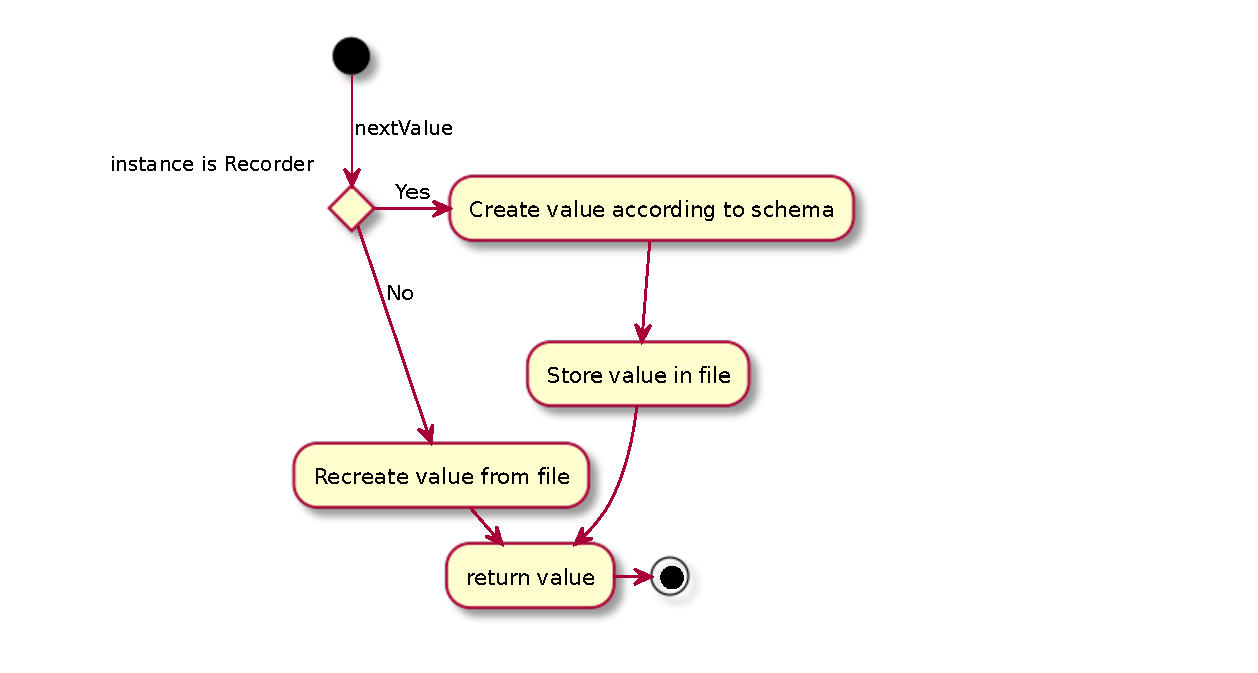
\includegraphics[width=\textwidth]{images/generalGeneratorWorkflow}
  \caption{Activity diagram roughly showing how the generators will work.}
  \label{fig:generalGeneratorWorkflow}
\end{figure}

\section{Execution Tool}
\label{ch:design:se:executionTool}
YCSB has a script to run one workload on one database.
We have many workloads and multiple databases,
therefore it would save us a lot of time during evaluation,
if the workloads are executed on all databases sequentially.

That could be implemented as a script that takes the databases and their parameters together with the workload description files and executes one after another.
The results should be saved in a specified folder.

\section{Evaluation Tool}
\label{ch:design:se:evaluationTool}
To gather the results another script should iterate through the result folders of each database and workload and collect the results in a file for further evaluation.
